% Beamer presentation
\documentclass[11pt,aspectratio=43,ignorenonframetext,t]{beamer}

% Presentation settings
\mode<presentation>{
  \usetheme[framenumber,titleframestart=1]{UoM_alex}
  \usefonttheme{professionalfonts} % using non standard fonts for beamer
  \usefonttheme{serif}
  \usepackage{fontspec}
  \setmainfont[Ligatures=TeX]{Arial}
}

% Handout settings
\mode<article>{
  \usepackage{fullpage}
  \usepackage{fontspec}
  \setmainfont[Ligatures=TeX]{Arial}
  \setlength{\parskip}{1.5\baselineskip} % correct beamer line spacings
  \setlength{\parindent}{0cm}
  \usepackage{enumitem}
  \setlist[itemize]{topsep=0pt}
}

 % Packages
\usepackage{graphicx}
\graphicspath{{./images/png}} % generic graphics path; overridden if necessary
\usepackage{amsmath}
\allowdisplaybreaks[1] % allow eqnarrays to break across pages
\usepackage{amssymb} 
\usepackage[HTML]{xcolor}
\definecolor{uomlinkblue}{HTML}{0071BC}
\usepackage{hyperref}
\hypersetup{
  colorlinks=true,
  linkcolor=uomlinkblue,
  filecolor=uomlinkblue,      
  urlcolor=uomlinkblue,
  pdflang={en-GB},
}
\usepackage[document]{ragged2e} % left aligned text for accessibility
\usepackage{tikz}
\usetikzlibrary{positioning, arrows, arrows.meta}
\usepackage{unicode-math} % unicode maths for accessibility
\usepackage{pdfcomment}   % for alt text for accessibility
\usepackage{rotating}     % allow portrait figures and tables
\usepackage{subfigure}    % allow matrices of figures
\usepackage{float}        % allows H option on floats to force here placement
\usepackage{multirow}     % allows merging of rows in tables
\usepackage{tabularx}     % allows fixed width tables
\usepackage{ctable}       % modifies \hline for use in table
\usepackage{bm}           % allow bold fonts in equations
\usepackage{pgf}          % allow graphics manipulation
\usepackage{etoolbox}
  
% Custom commands
\newcolumntype{Z}{>{\centering\arraybackslash}X}  % tabularx centered columns 

\makeatletter
  \DeclareRobustCommand{\em}
  {
    \@nomath\em
    \if b
      \expandafter\@car\f@series\@nil \normalfont
    \else
      \bfseries
    \fi
  }
\makeatother

\makeatletter
  \preto{\@verbatim}{\topsep=0pt \partopsep=0pt}
\makeatother

\def\checkmark{
  \tikz\fill[scale=0.4](0,.35) -- (.25,0) -- (1,.7) -- (.25,.15) -- cycle;
}

% Counters
\newcounter{example_number} % keep track of the example questions

% Frontmatter
\newcommand{\cmclecture}[1]{
  \title{Combinatorial Mesh Calculus (CMC): Lecture #1}
}
\author{
  Lectured by:
  \href{https://scholar.google.com/citations?user=x4R-snQAAAAJ&hl=en}
  {Dr. Kiprian Berbatov}$^1$\\
  \smallskip
  Lecture Notes Compiled by:
  \href{https://scholar.google.com/citations?user=CoIpITkAAAAJ&hl=en}
  {Muhammad Azeem}$^1$\\
  \smallskip
  Under the supervision of:
  \href{https://scholar.google.co.uk/citations?user=3nWJe5wAAAAJ&hl=en}
  {Prof. Andrey P. Jivkov}$^1$\\
  \smallskip
  {\tiny $^1$Department of Mechanical and Aerospace Engineering,
    The University of Manchester, Oxford Road, Manchester M13 9PL, UK}
}

% Special frames
\newcommand{\cmctitleframe}{
  \titlepage
  \begin{tikzpicture}[remember picture,overlay]
    \node[anchor=south east] at (current page.south east) {
      \href{https://youtube.com/@kipi.berbatov}{
        \includegraphics[width=1.5cm]{youtube-icon.png}
      }
    };
  \end{tikzpicture}
}
\newcommand{\cmcendframe}{
  \begin{figure}
    \centering
    \includegraphics[width=0.85\linewidth]{Thanks.png}
  \end{figure}
}

\cmclecture{3}
\date{15 October 2025}

\begin{document}

%========================= TITLE =========================
\begin{frame}
  \cmctitleframe
\end{frame}

\begin{frame}{Definition: Monoid Homomorphism}
\textbf{Definition.}  
Let $(M, *, e_M)$ and $(N, \circ, e_N)$ be monoids.  
A function \( f: M \to N \) is called a \textbf{monoid homomorphism} if it satisfies:

\begin{enumerate}
    \item \textbf{Compatibility with operation:}
    \[
        f(a * b) = f(a) \circ f(b), \quad \forall a,b \in M.
    \]
    \item \textbf{Preservation of identity:}
    \[
        f(e_M) = e_N.
    \]
\end{enumerate}

\textbf{Diagrammatic Representation:}
\centering
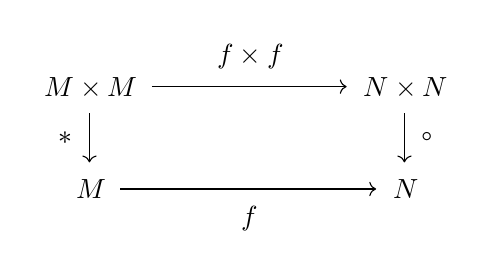
\begin{tikzpicture}[
    node distance=2.2cm and 4cm, % Vertical and Horizontal separation
    every node/.style={inner sep=6pt} 
]
    % 1. Define the nodes using explicit coordinates (similar to your error-prone code)
    \node (M) at (0,0) {$M\times M$};
    \node (N) at (4,0) {$N\times N$};
    \node (M1) at (0,-1.3) {$M$};
    \node (N1) at (4,-1.3) {$N$};
    
    % 2. Draw the arrows
    
    % M -> N (Horizontal: f x f)
    % FIX: Removed '>=Stealth' and used simple '->'
    \draw[->] (M) -- (N)
        node[midway, above] {$f\times f$};
    
    % M -> M1 (Vertical Left: *)
    % FIX: Removed '>=Stealth' and used simple '->'
    \draw[->] (M) -- (M1)
        node[midway, left] {$*$};
        
    % N -> N1 (Vertical Right: o)
    % FIX: Removed '>=Stealth' and used simple '->'
    \draw[->] (N) -- (N1)
        node[midway, right] {$\circ$};
        
    % M1 -> N1 (Bottom: f)
    % FIX: Removed '>=Stealth' and used simple '->'
    \draw[->] (M1) -- (N1)
        node[midway, below] {$f$};
        
\end{tikzpicture}
Commutativity of the diagram encodes: \( f(a*b) = f(a)\circ f(b). \)
\end{frame}

\begin{frame}{Examples of Monoid Homomorphisms}
\begin{block}{Example 1.} $(\mathbb{N}, +, 0)$ and $(\mathbb{N}, \times, 1)$  
Define \( f: \mathbb{N} \to \mathbb{N} \) by \( f(n) = 2^n. \)
\[
f(a+b) = 2^{a+b} = 2^a \cdot 2^b = f(a)f(b).
\]
Hence \(f\) is a monoid homomorphism.
\end{block} 
\begin{block}{Example 2.} $(\mathbb{R}, +, 0)$ and $(\mathbb{R}^+, \times, 1)$  
Define \( f(x) = e^x \).  
\[
f(x+y) = e^{x+y} = e^x e^y = f(x)f(y).
\]
Thus \(f\) is a monoid (and in fact group) homomorphism.
\end{block}  
\end{frame}

% ============================================================
\section{Group Homomorphisms}
% ============================================================

\begin{frame}{Definition: Group Homomorphism}
\vspace{-0.3cm}
\begin{block}{Definition.}  
Let $(G, *, e_G, i_G)$ and $(H, \circ, e_H, i_H)$ be groups.  
A map \( f:G \to H \) is called a \textbf{group homomorphism} if it satisfies:

\begin{enumerate}
    \item \( f(a*b) = f(a) \circ f(b) \) \hfill (operation preservation)
    \item \( f(e_G) = e_H \) \hfill (identity preservation)
    \item \( f(i_G(a)) = i_H(f(a)) \) \hfill (inverse preservation)
\end{enumerate}
\end{block}{}

\textbf{Diagrammatic form:}
\centering
\begin{tikzpicture}[
    node distance=2.2cm and 4cm, % Vertical and Horizontal separation
    every node/.style={inner sep=6pt} 
]
    % 1. Define the nodes using explicit coordinates 
    \node (G) at (0,0) {$G\times G$}; % Updated to G
    \node (H) at (4,0) {$H\times H$}; % Updated to H
    \node (G1) at (0,-1.3) {$G$};     % Updated to G
    \node (H1) at (4,-1.3) {$H$};     % Updated to H
    
    % 2. Draw the arrows
    
    % G -> H (Horizontal: f x f)
    \draw[->] (G) -- (H)
        node[midway, above] {$f\times f$};
    
    % G -> G1 (Vertical Left: *)
    \draw[->] (G) -- (G1)
        node[midway, left] {$*$};
        
    % H -> H1 (Vertical Right: o)
    \draw[->] (H) -- (H1)
        node[midway, right] {$\circ$};
        
    % G1 -> H1 (Bottom: f)
    \draw[->] (G1) -- (H1)
        node[midway, below] {$f$};
        
\end{tikzpicture}
The diagram commutes if \(f(a*b)=f(a)\circ f(b)\).
\end{frame}

\begin{frame}{Homomorphism Property Reduction}
\vspace{-0.3cm}
\begin{block}{Proposition.}  
Let \(f:G\to H\) be a function between groups.  
If \(f\) satisfies only
\[
f(a*b)=f(a)\circ f(b),
\]
then automatically:

\[
f(e_G)=e_H, \quad f(a^{-1})=f(a)^{-1}.
\]

\textbf{Proof.} $f(e_G) = f(e_G * e_G) = f(e_G)\circ f(e_G)
\Rightarrow f(e_G) = e_H.$ \\
Next, \[e_H = f(e_G) = f(a*a^{-1}) = f(a)\circ f(a^{-1}) \Rightarrow f(a^{-1}) = f(a)^{-1}. \quad\square
\]

\textbf{Hence:} Only property (1) is needed to check; others follow automatically.
\end{block}
\end{frame}

% ============================================================
\section{Isomorphisms}
% ============================================================

\begin{frame}{Isomorphism of Monoids or Groups}
\vspace{-0.3cm}
\begin{block}{Definition.}  
Let $(X, *, e_X)$ and $(Y, \circ, e_Y)$ be monoids (or groups).  
A map \(f:X\to Y\) is called an \emph{isomorphism} if:
\begin{enumerate}
    \item \(f\) is a homomorphism;
    \item \(f\) is bijective;
    \item \(f^{-1}\) is also a homomorphism.
\end{enumerate}
\end{block}
\vspace{-0.3cm}
\begin{block}{Remark.}
If \(f\) is bijective and satisfies \(f(a*b)=f(a)\circ f(b)\), then its inverse \(f^{-1}\) automatically respects the operations.  
Hence, bijectivity is enough to guarantee isomorphism.

\textbf{Notation:}
\[
(X, *, e_X) \cong (Y, \circ, e_Y).
\]
Read as “\(X\) and \(Y\) are isomorphic as monoids (or groups).”
\end{block}
\end{frame}

\begin{frame}{Example: Exponential Isomorphism}
\vspace{-0.3cm}
\begin{block}{Example.}
\[
(\mathbb{R}, +, 0) \xrightarrow{\,f(x)=e^x\,} (\mathbb{R}^+, \times, 1).
\]
Check:
\[
f(x+y)=e^{x+y}=e^x e^y=f(x)f(y),\quad f(0)=1.
\]
Inverse map: \(f^{-1}(y)=\ln(y)\).  
Then
\[
\ln(xy)=\ln(x)+\ln(y).
\]
Hence both \(f\) and \(f^{-1}\) are homomorphisms.

\[
(\mathbb{R}, +) \cong (\mathbb{R}^+, \times).
\]
\end{block}
\end{frame}


\begin{frame}{Subgroup}
\begin{block}{Definition.}  
Let $(G, *, e, i)$ be a group. A subset \(H \subseteq G\) is a \emph{subgroup} of \(G\), if it is a group with the same operations restricted to $H$. In other words, we need:

\begin{enumerate}
  \item \(e \in H\) \hfill (contains identity),
  \item \(\forall a,b \in H,\; a*b \in H\) \hfill (closed under operation),
  \item \(\forall a \in H,\; i(a) \in H\) \hfill (closed under inverses).
\end{enumerate}

We denote it as \(H \leq G.\)
\end{block}
\end{frame}

\begin{frame}{Simplified Subgroup Test}
\begin{block}{Remark.}  
The above three properties can be reduced to a single condition:
\[
\forall a,b \in H,\quad a * b^{-1} \in H.
\]

\textbf{Proof.}
\begin{itemize}
  \item Let \(a=b=e\): gives \(e\in H\).
  \item For \(a,b\in H\), \(b^{-1}\in H\) so \(a*b^{-1}\in H \Rightarrow\) closure.
  \item Taking \(a=e\), \(e*b^{-1}=b^{-1}\in H\) gives closure under inverses.
\end{itemize}

Hence condition (4) implies all three original subgroup properties. \(\square\)
\end{block}
\end{frame}

% ============================================================
\section{Examples of Subgroups}
% ============================================================

\begin{frame}{Example 1: $(\mathbb{Z}, +)$ and $n\mathbb{Z}$}
\begin{block}{}
    Let \(G=(\mathbb{Z}, +, 0)\) and \(H = n\mathbb{Z} = \{nk : k\in \mathbb{Z}\}.\)

\textbf{Proof.}
\begin{itemize}
  \item \(0 = n\cdot 0 \in n\mathbb{Z}\).
  \item For \(a=nk_1, b=nk_2 \in n\mathbb{Z}\), \(a-b = n(k_1-k_2)\in n\mathbb{Z}\).
\end{itemize}
Hence \(H\) is a subgroup of \(G.\)

\[
n\mathbb{Z} \le \mathbb{Z}.
\]
\textbf{Diagram:}
\[
\mathbb{Z} \supset 2\mathbb{Z} \supset 4\mathbb{Z} \supset 8\mathbb{Z} \supset \cdots
\]
Chain of nested subgroups under divisibility.
\end{block}

\end{frame}

\begin{frame}{Example 2: $SL_n(\mathbb{R})$ in $GL_n(\mathbb{R})$}
\begin{block}{}
Let
\[
G = GL_n(\mathbb{R}) = \{A\in M_{n\times n}(\mathbb{R}) \mid \det(A)\ne 0\},
\]
\[
H = SL_n(\mathbb{R}) = \{A\in G \mid \det(A)=1\}.
\]

\textbf{Proof.}
\begin{itemize}
  \item \(I_n \in H\) since \(\det(I_n)=1.\)
  \item If \(A,B \in H\), then \(\det(AB)=\det(A)\det(B)=1\cdot1=1 \Rightarrow AB\in H.\)
  \item If \(A\in H\), then \(\det(A^{-1}) = 1/\det(A) = 1 \Rightarrow A^{-1}\in H.\)
\end{itemize}

Hence \(SL_n(\mathbb{R}) \le GL_n(\mathbb{R})\).
\end{block}
\end{frame}

% ============================================================
\begin{frame}{Two Views: $\mathbf{GL_n(\mathbb{R})}$, $\mathbf{SL_n(\mathbb{R})}$}
\vspace{-0.3cm}
\centering
\begin{columns}
\column{0.45\textwidth}
\vspace{-0.3cm}
\begin{block}{Subgroup Hierarchy (Inclusion)}
\begin{center}
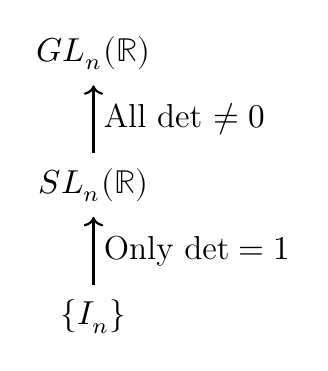
\begin{tikzpicture}[node distance=1.0cm, every node/.style={font=\large}]
\node (G) at (0,0) {$GL_n(\mathbb{R})$};
\node (H) [below=of G] {$SL_n(\mathbb{R})$};
\node (K) [below=of H] {$\{I_n\}$};
\draw[->, thick, shorten >= 2pt, shorten <= 2pt] (H)--(G) node[midway, right] {All det $\ne 0$};
\draw[->, thick, shorten >= 2pt, shorten <= 2pt] (K)--(H) node[midway, right] {Only $\det=1$};
\end{tikzpicture}
\end{center}
\vspace*{0.5em}
\alert{Idea:} $\mathbf{SL_n(\mathbb{R})}$ is a subgroup of $\mathbf{GL_n(\mathbb{R})}$.
\end{block}

% --- Column 2: Short Exact Sequence (The original concept) ---
\column{0.55\textwidth}
\vspace{-0.3cm}

\begin{alertblock}{Key Idea}
The special linear group, $\mathbf{SL_n(\mathbb{R})}$, is the set of matrices where the determinant is exactly 1. This means it's the \textbf{kernel} (or null space) of the determinant function, and the whole relationship reveals that the quotient group $\mathbf{GL_n(\mathbb{R})} / \mathbf{SL_n(\mathbb{R})}$ is isomorphic to $\mathbf{\mathbb{R}^*}$ (all non-zero real numbers).
\end{alertblock}
\end{columns}

\end{frame}

\begin{frame}{Two Views: $\mathbf{GL_n(\mathbb{R})}$, $\mathbf{SL_n(\mathbb{R})}$}

\begin{block}{Short Exact Sequence (Quotient)}
\begin{center}
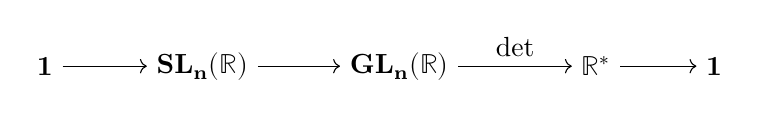
\begin{tikzpicture}[scale=1.0, every node/.style={font=\normalsize}]
% Define the nodes
\node (one) at (-2.5, 0) {$\mathbf{1}$};
\node (sl) at (-0.5, 0) {$\mathbf{SL_n(\mathbb{R})}$};
\node (gl) at (2, 0) {$\mathbf{GL_n(\mathbb{R})}$};
\node (f) at (4.5, 0) {$\mathbf{\mathbb{R}^*}$};
\node (one2) at (6, 0) {$\mathbf{1}$};

% Draw the maps
\draw[->] (one) -- (sl);
\draw[->] (sl) -- (gl);
\draw[->] (gl) -- node[above] {$\det$} (f);
\draw[->] (f) -- (one2);
\end{tikzpicture}
\end{center}
\vspace*{0.5em}
\textbf{The Sequence:} $1 \to SL_n(\mathbb{R}) \to GL_n(\mathbb{R}) \xrightarrow{\det} \mathbb{R}^* \to 1$
\end{block}


\end{frame}


\begin{frame}{Distributivity}
\begin{block}{Definition.}  
Let $(R,+,.)$ be a set with two binary operations: addition $(+)$ and multiplication $(.)$.  
We say multiplication is \emph{distributive over addition} if for all $a,b,c\in R$:
\[
a.(b+c) = a.b + a.c \quad \text{and} \quad (a+b).c = a.c + b.c.
\]
\end{block}
\begin{block}{Remark:}
This property ensures addition and multiplication interact consistently-fundamental to defining rings.
\end{block}
\end{frame}


\begin{frame}{Ring}
\begin{block}{Definition}  
A \emph{ring} is a set \(R\) together with two binary operations \(+\) (addition) and \(.\) (multiplication) such that the following properties hold for all \(a,b,c\in R\):

\begin{enumerate}
  \item \(a+(b+c) = (a+b)+c\) \hfill (Associativity of addition)
  \item \(a+b = b+a\) \hfill (Commutativity of addition)
  \item There exists \(0 \in R\) such that \(a+0=a=0+a\) \hfill (Additive identity)
  \item For every \(a\in R\), there exists \((-a)\in R\) such that \(a+(-a)=0\) \hfill (Additive inverse)
  \item \(a.(b.c)=(a.b).c\) \hfill (Associativity of multiplication)
  \item \(a.(b+c)=a.b+a.c\) and \((a+b).c=a.c+b.c\) \hfill (Distributivity)
\end{enumerate}

Then \((R,+)\) is an abelian group and \((R,.)\) is a semigroup.
\end{block}
\end{frame}

\begin{frame}{Refinements of Rings}
\vspace{-0.3cm}
\begin{block}{Definition (Commutative Ring).}  
A ring \((R,+,.)\) is called \emph{commutative} if \(a.b=b.a\) for all \(a,b\in R.\)
\end{block}
\vspace{-0.3cm}
\begin{block}{Definition (Ring with Unity).}  
A ring having an element \(1\) such that \(1.a=a.1=a\) for all \(a\in R\) is called a \emph{ring with unity.}
\end{block}
\vspace{-0.3cm}
\begin{block}{Definition (Division Ring).}  
A ring with unity where every nonzero element has a multiplicative inverse, but multiplication need not be commutative.
\end{block}
\vspace{-0.3cm}
\begin{block}{Definition (Field).}  
A \emph{field} is a commutative division ring:  
\[
\forall a\neq0,\,\exists a^{-1}\in R:\,a.a^{-1}=a^{-1}.a=1.
\]
\end{block}
\end{frame}

\begin{frame}{From Ring to Field: Structural Properties}
\vspace{-0.5cm}
\begin{block}{}
    A structure $(R,+,.,0,1,-)$ satisfies the following ten axioms:

\begin{columns}[t]
\column{0.52\textwidth}
\textbf{Additive properties:}
\begin{enumerate}
\item $a+(b+c)=(a+b)+c$
\item $a+b=b+a$
\item $\exists\,0\in R$ s.t. $a+0=a$
\item $\forall a\in R, \exists (-a)$ s.t. $a+(-a)=0$
\end{enumerate}

\column{0.45\textwidth}
\textbf{Multiplicative and mixed properties:}
\begin{enumerate}
\setcounter{enumi}{4}
\item $a.(b.c)=(a.b).c$
\item $a.(b+c)=a.b+a.c$
\item $(a+b).c=a.c+b.c$
\item $\exists\,1\in R$ s.t. $a.1=1.a=a$
\item $\forall a\neq0, \exists a^{-1}$ s.t. $a.a^{-1}=1$
\item $a.b=b.a$
\end{enumerate}
\end{columns}
\vspace{-0.7cm}
\textbf{Observation:}
\begin{itemize}
  \item 1–7 → Ring
  \item 1–8 → Ring with Unity
  \item 1–9 → Division Ring
  \item 1–10 → Field
\end{itemize}
\end{block}
\end{frame}

% ============================================================
\section{Examples of Rings and Fields}
% ============================================================

\begin{frame}{Examples}
\begin{block}{Ring-like Structures}
  \begin{enumerate}
      \item $(\mathbb{Z},+,.)$ — commutative ring with unity $1$.
      \item $(2\mathbb{Z},+,.)$ — commutative ring without unity.
\item $(\mathbb{N},+,.)$ — semiring (no additive inverses).
\item $(\mathbb{Q},+,.)$ — field.
\item $(\mathbb{R},+,.)$ — field.
\item $(\mathbb{C},+,.)$ — field.
  \end{enumerate}  
\end{block}

\end{frame}

\begin{frame}{Examples}
\begin{block}{Non-Commutative Rings and Division Rings}
\begin{enumerate}
\item[7] $(M_{n\times n}(\mathbb{R}), +, .)$ — ring with unity, not commutative for $n>1$.  
\item[8] $(M_{n\times n}(\mathbb{Z}), +, .)$ — commutative in addition only.  
\item[9] $(\mathbb{H},+,.)$ — quaternions: division ring, not commutative.  
\[
\mathbb{H}=\{a+bi+cj+dk \mid a,b,c,d\in\mathbb{R}\},\quad i^2=j^2=k^2=ijk=-1.
\]
\item[10] $(\mathbb{Z}_n, +, \cdot)$ — commutative ring with unity; field iff $n$ prime.  
\item[11]  Polynomial rings $(\mathbb{R}[x], +, .)$ — commutative ring with unity.  
\item[12]  Continuous functions $(C([0,1]), +, .)$ — commutative ring with unity.
\end{enumerate} 
\end{block}
 
\end{frame}

% ============================================================
\section{Function Rings}
% ============================================================

\begin{frame}{Function Ring $R^X$}
\begin{block}{Definition}
    Let $R$ be a commutative ring with unity and $X$ a nonempty set.

Define
\[
R^X = \{ f : X \to R \}.
\]
Define operations:
\[
(f \tilde{+} g)(x) = f(x) + g(x), \qquad (f \, \tilde{\cdot}\,  g)(x) = f(x)\cdot g(x).
\]
Define $\tilde{0}(x)=0$ and $\tilde{1}(x)=1$ for all $x\in X$.

\textbf{Claim:} $(R^X, \tilde{+}, \, \tilde{\cdot}\, , \tilde{0}, \tilde{1})$ is a commutative ring with unity.
\end{block}
\end{frame}

\begin{frame}{$(R^X, \tilde{+}, \, \tilde{\cdot}\, )$ - Commutative Ring with Unity}
\textbf{Proof (Sketch):}\\
\textbf{Addition:} For all $f,g,h\in R^X$,
  \[
  (f\tilde{+}(g\tilde{+}h))x = fx + (gx+hx) = (fx+gx)+hx = ((f\tilde{+}g)\tilde{+}h)x.
  \]
  Hence associative. Commutativity and additive inverse follow pointwise.\\
  \textbf{Multiplication:}
  \[
  (f\, \tilde{\cdot}\, (g\, \tilde{\cdot}\, h))x = fx(gxhx) = (fxgx)hx = ((f\, \tilde{\cdot}\, g)\, \tilde{\cdot}\, h)x.
  \]
  \\ \textbf{Distributivity:}
  \[
  (f\, \tilde{\cdot}\, (g\tilde{+}h))x=fx(gx+hx)=fxgx+fxhx=(f\, \tilde{\cdot}\, g\tilde{+}f\, \tilde{\cdot}\, h)x.
  \]
  \\ \textbf{Unity:} $\tilde{1}x=1$ satisfies $f\, \tilde{\cdot}\, \tilde{1}=f$.\\

Hence, all ring axioms hold pointwise. $\square$
\end{frame}


\begin{frame}{(1): Proof that $R^X$ is a Commutative Ring}
\begin{block}{Solution.}
The verification above confirms:
\[
(R^X, \tilde{+}, \, \tilde{\cdot}\, , \tilde{0}, \tilde{1})
\]
inherits all ring properties from $R$ under pointwise operations.  
Hence, $R^X$ is a \emph{commutative ring with unity.}
\end{block}
\end{frame}

% ============================================================
\begin{frame}{(2): Ring Structure on $\mathbb{Q}$ via $a*b=a+b+ab$}
\textbf{Define:} $a*b=a+b+ab$ for $a,b\in\mathbb{Q}$.

\textbf{Check Associativity:}
\[
a*(b*c) = a+(b+c+bc)+a(b+c+bc) = a+b+c+ab+ac+bc+abc.
\]
\[
(a*b)*c = (a+b+ab)+c+(a+b+ab)c = a+b+c+ab+ac+bc+abc.
\]
Hence associative. $\checkmark$

\textbf{Unity:} find $e$ s.t. $a*e=a$.  
\[
a+e+ae=a \Rightarrow e(1+a)=0 \Rightarrow e=0.
\]
So $0$ is unity. $\checkmark$

\textbf{Group of units:}  
$a*b=0 \Rightarrow a+b+ab=0 \Rightarrow (1+a)(1+b)=1$.  
Hence unit $a$ exists iff $1+a\ne0$, and inverse is $b=-a/(1+a)$.  
Thus units: $\mathbb{Q}\setminus\{-1\}.$
\end{frame}

% ============================================================
\begin{frame}{(3): Real Interval Group with Parameter $k>0$}
Define for $a,b\in(-k,k)$:
\[
a*b=\frac{a+b}{1+kb}.
\]
\textbf{Closure:}
If $a,b\in(-k,k)$, then $|a*b|<k$ (exercise: verify using $|a+b|<2k$ and $1+kb>1-k^2>0$).

\textbf{Associativity:}  
Compute:
\[
a*(b*c)=\frac{a+\frac{b+c}{1+kc}}{1+k\frac{b+c}{1+kc}}=\frac{a(1+kc)+b+c}{1+k(a+b+c)+k^2(bc+ac+ab)}.
\]
A tedious but direct algebra shows symmetry, hence associative. $\checkmark$

\textbf{Identity:} $0$, since $a*0=\frac{a+0}{1+0}=a$. $\checkmark$  
\textbf{Inverse:} $a^{-1}=-\frac{a}{1+ka}$. $\checkmark$

Hence \(((-k,k),*,0)\) is a group (nonlinear addition law, used in hyperbolic geometry).
\end{frame}

% ============================================================
\begin{frame}{(4): Constructing a Ring on $\mathbb{R}^2$}
Define operations for $(a,b),(c,d)\in\mathbb{R}^2$:
\[
(a,b)\tilde{+}(c,d)=(a+c,b+d),\quad
(a,b)\, \tilde{\cdot}\, (c,d)=(ac,\,bc+ad).
\]

\textbf{Check Ring Properties:}
\begin{itemize}
  \item Addition is componentwise abelian group: $\checkmark$
  \item Multiplication associative:  
    \((a,b)\, \tilde{\cdot}\, ((c,d)\, \tilde{\cdot}\, (e,f)) = (a(b+c)+\dots)\) (verify explicitly). $\checkmark$
  \item Distributivity holds componentwise: $\checkmark$
  \item Unity element: $(1,0)$ since
  \[
  (a,b)\, \tilde{\cdot}\, (1,0)=(a,b).
  \]
  \item Commutativity:  
  \((a,b)\, \tilde{\cdot}\, (c,d)=(ac,bc+ad)=(c,a)\, \tilde{\cdot}\, (a,b)\). $\checkmark$
\end{itemize}
Hence $(\mathbb{R}^2,\tilde{+},\, \tilde{\cdot}\, )$ is a commutative ring with unity $(1,0)$.
\end{frame}

\begin{frame}{Algebraic Structure of $\mathbb{R}^2$ with Custom Multiplication}
\vspace{-0.3cm}
\begin{center}
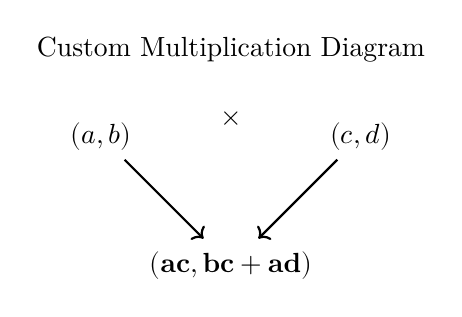
\begin{tikzpicture}[scale=1.1, every node/.style={font=\normalsize}]
\node (a) at (0,0) {$(a,b)$};
\node (b) at (3,0) {$(c,d)$};
\node (times) at (1.5, 0.2) {$\mathbf{\times}$};
\node (p) at (1.5,-1.5) {$\mathbf{(ac, bc+ad)}$};
\node at (1.5,1) {Custom Multiplication Diagram};
\draw[->, thick, shorten >= 2pt] (a)--(p);
\draw[->, thick, shorten >= 2pt] (b)--(p);
\end{tikzpicture}
\end{center}
\begin{block}{Interpretation and Clarification}
This diagram illustrates the algebraic structure of $\mathbb{R}^2$ under the explicit multiplication rule:
$$(a, b) * (c, d) = (ac, bc + ad)$$
\end{block}
\end{frame}

\begin{frame}{Algebraic Structure of $\mathbb{R}^2$}
\vspace{-0.3cm}
\begin{block}{Interpretation and Clarification}
This diagram illustrates the algebraic structure of $\mathbb{R}^2$ under the explicit multiplication rule:
$(a, b) * (c, d) = (ac, bc + ad)$
\begin{itemize}
    \item With standard vector addition, this operation defines a \textbf{Ring} structure on $\mathbb{R}^2$.
    \item \textbf{Note on Affine Transformations:} While the multiplication is commutative in the second component ($bc+ad$), the standard way to model affine transformations $f(x) = ax+b$ is through composition, which results in the pair:
    $$(a,b) \circ (c,d) = (\mathbf{ac}, \mathbf{ad+b})$$
    \item Your rule and the affine group rule are related, but they define different algebraic structures!
\end{itemize}
\end{block}
\end{frame}

% ============================================================
\begin{frame}{Summary}
\vspace{-0.3cm}
\begin{itemize}
  \item Introduced distributivity linking addition and multiplication, then defined ring, commutative ring, ring with unity, division ring, and field.
\item Outlined 10 structural axioms progressing from semiring to field.
\item Provided 12 diverse examples, including quaternions.
\item Proved $(R^X,\tilde{+},\, \tilde{\cdot}\, )$ is a commutative ring with unity.
\item Solved four constructive problems demonstrating new ring-like and group structures.
\item Defined monoid and group homomorphisms with formal diagrams; proved that for group homomorphisms, one property implies the rest.
\item Defined and illustrated isomorphisms with exponential–log example.
\item Defined subgroup and proved simplified test using \(a*b^{-1}\); worked examples: $(\mathbb{Z},+)$ and $(GL_n(\mathbb{R}),\times)$.
\end{itemize}
\end{frame}

\begin{frame}{Thanks}
  \cmcendframe
\end{frame}

\end{document}
